\documentclass[aspectratio=169,11pt]{beamer}

% Theme
\usetheme{default}
\setbeamertemplate{navigation symbols}{}
\setbeamertemplate{footline}{%
  \hfill\insertframenumber/\inserttotalframenumber\hspace*{4pt}\vspace{2pt}%
}

% Packages
\usepackage{lmodern}
\usepackage[most]{tcolorbox}
\usepackage{listings}
\usepackage{tikz}
\usetikzlibrary{arrows.meta,positioning,shapes.geometric,fit,backgrounds}
\usepackage{booktabs}
\usepackage{hyperref}
% fontawesome5 not available in this TeX distribution

% Colors
\definecolor{lcgreen}{HTML}{2E7D32}
\definecolor{lcblue}{HTML}{1565C0}
\definecolor{lcorange}{HTML}{EF6C00}
\definecolor{lcred}{HTML}{C62828}
\definecolor{codebg}{HTML}{F5F5F5}
\definecolor{docgray}{gray}{0.55}

% tcolorbox styles - compact padding
\newtcolorbox{conceptbox}[1][]{colback=yellow!20,colframe=yellow!60!black,title=#1,fonttitle=\bfseries,top=2pt,bottom=2pt,left=4pt,right=4pt}
\newtcolorbox{warningbox}[1][]{colback=red!15,colframe=red!60!black,title=#1,fonttitle=\bfseries,top=2pt,bottom=2pt,left=4pt,right=4pt}
\newtcolorbox{tipbox}[1][]{colback=green!10,colframe=green!50!black,title=#1,fonttitle=\bfseries,top=2pt,bottom=2pt,left=4pt,right=4pt}
\newtcolorbox{codebox}[1][]{colback=blue!10,colframe=blue!40!black,title=#1,fonttitle=\bfseries,top=2pt,bottom=2pt,left=4pt,right=4pt}

% Listings style
\lstset{
  basicstyle=\ttfamily\scriptsize,
  backgroundcolor=\color{codebg},
  breaklines=true,
  frame=single,
  rulecolor=\color{blue!40!black},
  keywordstyle=\color{lcblue}\bfseries,
  stringstyle=\color{lcgreen},
  commentstyle=\color{docgray}\itshape,
  language=Python,
  showstringspaces=false,
  tabsize=2,
  xleftmargin=2pt,
  xrightmargin=2pt,
  aboveskip=2pt,
  belowskip=2pt,
}

% Compact itemize spacing
\setlength{\itemsep}{1pt}
\setlength{\parsep}{0pt}
\setlength{\parskip}{0pt}

% Doc reference command
\newcommand{\docref}[1]{{\scriptsize\color{docgray}[Docs: #1]}}

\title{\textbf{LangChain} --- Overview \& Architecture}
\subtitle{Section 00: Why LangChain Exists and How It Fits Together}
\author{LangChain v1.2.x Study Guide}
\date{March 2026}

\begin{document}

% ============================================================
\begin{frame}
\titlepage
\end{frame}

% ============================================================
\begin{frame}{What You Will Learn}
\begin{conceptbox}[Section Objectives]
By the end of this section, you will understand:
\begin{itemize}\setlength{\itemsep}{1pt}
  \item What problem LangChain solves and why it exists
  \item The LangChain ecosystem: LangChain, LangGraph, LangSmith
  \item The package architecture and how modules relate
  \item How to install and configure LangChain
  \item Where LangChain fits relative to alternatives
\end{itemize}
\end{conceptbox}

\vspace{0.2cm}
\textbf{Prerequisites:} Basic Python knowledge. No prior LangChain experience needed.

\docref{langchain.com/docs}
\end{frame}

% ============================================================
\begin{frame}{Mental Model: The LangChain Universe}
\begin{center}
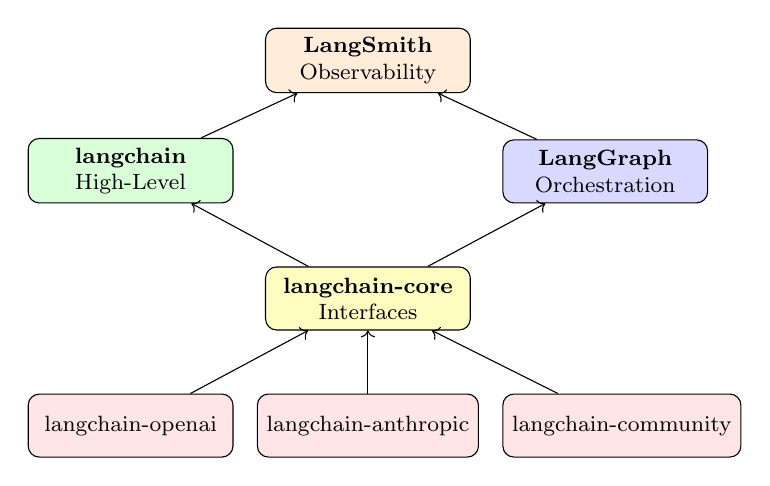
\begin{tikzpicture}[
  node distance=1.0cm,
  box/.style={rectangle, rounded corners, draw, minimum width=2.6cm, minimum height=0.8cm, align=center, font=\footnotesize},
  every edge/.style={draw, -{Stealth[length=5pt]}},
]
  \node[box, fill=yellow!25] (core) {\textbf{langchain-core}\\Interfaces};
  \node[box, fill=green!15, above left=0.8cm and 0.4cm of core] (lc) {\textbf{langchain}\\High-Level};
  \node[box, fill=blue!15, above right=0.8cm and 0.4cm of core] (lg) {\textbf{LangGraph}\\Orchestration};
  \node[box, fill=orange!15, above=2.2cm of core] (ls) {\textbf{LangSmith}\\Observability};
  \node[box, fill=red!10, below left=0.8cm and 0.4cm of core] (oai) {langchain-openai};
  \node[box, fill=red!10, below=0.8cm of core] (anth) {langchain-anthropic};
  \node[box, fill=red!10, below right=0.8cm and 0.4cm of core] (comm) {langchain-community};

  \draw[->] (core) -- (lc);
  \draw[->] (core) -- (lg);
  \draw[->] (lc) -- (ls);
  \draw[->] (lg) -- (ls);
  \draw[->] (oai) -- (core);
  \draw[->] (anth) -- (core);
  \draw[->] (comm) -- (core);
\end{tikzpicture}
\end{center}
\docref{docs.langchain.com/oss/python/concepts}
\end{frame}

% ============================================================
\begin{frame}{The Problem: Why LangChain?}

\textbf{Building LLM applications without a framework means:}

\begin{itemize}\setlength{\itemsep}{2pt}
  \item Writing custom glue code for every LLM provider
  \item Manually managing prompt templates, output parsing, error handling
  \item Reinventing conversation memory, tool calling, retrieval patterns
  \item No standardized way to compose, test, or observe your pipelines
\end{itemize}

\vspace{0.2cm}

\begin{conceptbox}[LangChain's Value Proposition]
LangChain provides \textbf{standardized interfaces} for LLM components and \textbf{composable primitives} for chaining them together --- so you can swap providers, add tools, and build agents without rewriting your application.
\end{conceptbox}
\end{frame}

% ============================================================
\begin{frame}{What LangChain Is\ldots}

\begin{columns}[T]
\begin{column}{0.48\textwidth}
\begin{tipbox}[LangChain IS]
\begin{itemize}\setlength{\itemsep}{1pt}
  \item A framework for composing LLM calls
  \item An abstraction layer over providers
  \item A toolkit for agents, RAG, tools
  \item An orchestration platform (via LangGraph)
  \item Provider-agnostic by design
\end{itemize}
\end{tipbox}
\end{column}

\begin{column}{0.48\textwidth}
\begin{warningbox}[LangChain is NOT]
\begin{itemize}\setlength{\itemsep}{1pt}
  \item An LLM itself
  \item A hosted AI service
  \item A UI framework
  \item Required for all LLM apps
  \item A replacement for understanding LLMs
\end{itemize}
\end{warningbox}
\end{column}
\end{columns}
\end{frame}

% ============================================================
\begin{frame}{When to Use LangChain}

\begin{tipbox}[Good Fit]
Use LangChain when you need \textbf{multi-step LLM workflows}, \textbf{tool calling}, \textbf{retrieval}, or \textbf{agents}. It shines when you want provider flexibility and production observability.
\end{tipbox}

\vspace{0.3cm}

\begin{warningbox}[May Be Overkill]
For a single LLM API call with no chaining, the raw provider SDK (e.g., \texttt{openai} or \texttt{anthropic}) may be simpler and more direct.
\end{warningbox}
\end{frame}

% ============================================================
\begin{frame}{The Ecosystem at a Glance}

\begin{center}
\renewcommand{\arraystretch}{1.3}
\footnotesize
\begin{tabular}{lp{4.5cm}p{3.5cm}}
\toprule
\textbf{Component} & \textbf{Purpose} & \textbf{When You Need It} \\
\midrule
\texttt{langchain-core} & Base interfaces (Runnables, Messages, Tools) & Always (auto-installed) \\
\texttt{langchain} & High-level chains, agents, retrieval & Most applications \\
\texttt{langgraph} & Graph-based agent orchestration & Complex agent workflows \\
\texttt{langsmith} & Tracing, evaluation, monitoring & Testing \& production \\
\texttt{langchain-openai} & OpenAI integration & If using OpenAI models \\
\texttt{langchain-anthropic} & Anthropic integration & If using Claude models \\
\texttt{langchain-community} & 700+ third-party integrations & As needed \\
\bottomrule
\end{tabular}
\end{center}

\docref{docs.langchain.com/oss/python/concepts/architecture}
\end{frame}

% ============================================================
\begin{frame}[fragile]{Installation}

\begin{codebox}[Basic Installation]
\begin{lstlisting}
# Core + high-level features
pip install langchain

# Add provider packages as needed
pip install langchain-openai       # OpenAI models
pip install langchain-anthropic    # Claude models
pip install langchain-google-genai # Gemini models

# Optional: orchestration & observability
pip install langgraph
pip install langsmith
\end{lstlisting}
\end{codebox}

\vspace{0.15cm}

\begin{warningbox}[Version Note]
LangChain v1.2.x is the current stable release. The legacy \texttt{langchain-classic} package is \textbf{not recommended} for new projects.
\end{warningbox}
\end{frame}

% ============================================================
\begin{frame}[fragile]{Environment Setup}

\begin{codebox}[API Key Configuration]
\begin{lstlisting}
# Option 1: Environment variables (recommended)
export OPENAI_API_KEY="sk-..."
export ANTHROPIC_API_KEY="sk-ant-..."
export LANGSMITH_API_KEY="lsv2_..."  # optional

# Option 2: Pass directly in code
from langchain_openai import ChatOpenAI
llm = ChatOpenAI(api_key="sk-...")
\end{lstlisting}
\end{codebox}

\vspace{0.15cm}

\begin{tipbox}[Best Practice]
Use environment variables or a \texttt{.env} file with \texttt{python-dotenv}. Never hardcode API keys in source code.
\end{tipbox}
\end{frame}

% ============================================================
\begin{frame}[fragile]{Your First LangChain Program}

\begin{codebox}[Hello LangChain]
\begin{lstlisting}
from langchain_openai import ChatOpenAI
from langchain_core.messages import HumanMessage

# 1. Initialize a chat model
llm = ChatOpenAI(model="gpt-4o")

# 2. Send a message
response = llm.invoke([
    HumanMessage(content="What is LangChain in one sentence?")
])

# 3. Print the result
print(response.content)
\end{lstlisting}
\end{codebox}

\vspace{0.1cm}
\textbf{Key observation:} The \texttt{invoke()} method is the universal interface --- every LangChain component supports it.
\end{frame}

% ============================================================
\begin{frame}{Package Architecture Deep Dive}

\begin{center}
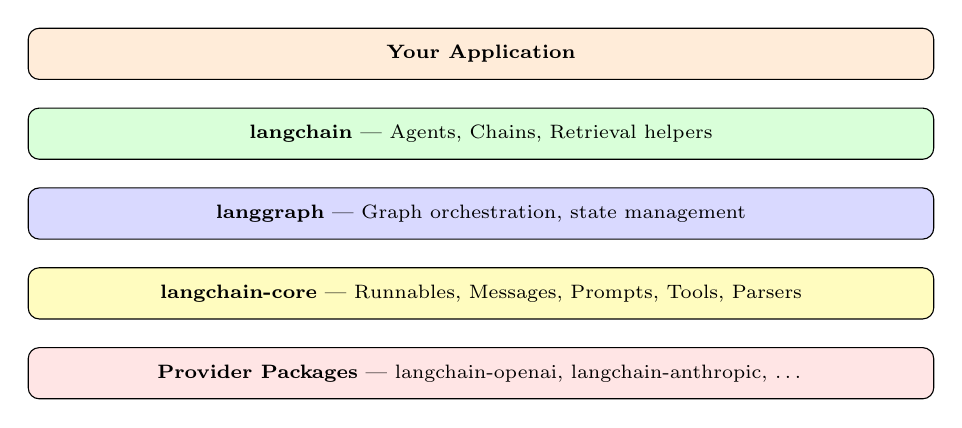
\begin{tikzpicture}[
  node distance=0.35cm,
  layer/.style={rectangle, rounded corners, draw, minimum width=11.5cm, minimum height=0.65cm, align=center, font=\scriptsize},
]
  \node[layer, fill=orange!15] (app) {\textbf{Your Application}};
  \node[layer, fill=green!15, below=of app] (lc) {\textbf{langchain} --- Agents, Chains, Retrieval helpers};
  \node[layer, fill=blue!15, below=of lc] (lg) {\textbf{langgraph} --- Graph orchestration, state management};
  \node[layer, fill=yellow!25, below=of lg] (core) {\textbf{langchain-core} --- Runnables, Messages, Prompts, Tools, Parsers};
  \node[layer, fill=red!10, below=of core] (providers) {\textbf{Provider Packages} --- langchain-openai, langchain-anthropic, \ldots};
\end{tikzpicture}
\end{center}

\vspace{0.1cm}
\begin{conceptbox}[Key Principle]
Dependencies flow \textbf{downward}: \texttt{langchain} depends on \texttt{langchain-core}, never the reverse.
\end{conceptbox}
\end{frame}

% ============================================================
\begin{frame}{Core Abstractions Preview}

\begin{center}
\renewcommand{\arraystretch}{1.2}
\footnotesize
\begin{tabular}{lp{7.5cm}}
\toprule
\textbf{Abstraction} & \textbf{What It Does} \\
\midrule
\textbf{Runnable} & Universal protocol: anything with \texttt{invoke()}, \texttt{batch()}, \texttt{stream()} \\
\textbf{ChatModel} & Wraps an LLM provider; takes messages, returns messages \\
\textbf{PromptTemplate} & Formats variables into prompts \\
\textbf{OutputParser} & Converts raw LLM text into structured data \\
\textbf{Tool} & A function the LLM can decide to call \\
\textbf{Retriever} & Fetches relevant documents given a query \\
\textbf{Chain (LCEL)} & A pipeline of Runnables composed with \texttt{|} \\
\textbf{Agent} & An LLM that plans and executes tool calls in a loop \\
\bottomrule
\end{tabular}
\end{center}

\vspace{0.15cm}
\textit{Each of these is covered in depth in subsequent sections.}

\docref{docs.langchain.com/oss/python/concepts}
\end{frame}

% ============================================================
\begin{frame}{The Runnable Protocol}

\begin{conceptbox}[The Universal Interface]
Every LangChain component implements the \textbf{Runnable} protocol:
\begin{itemize}\setlength{\itemsep}{1pt}
  \item \texttt{invoke(input)} --- Process a single input
  \item \texttt{batch([inputs])} --- Process multiple inputs in parallel
  \item \texttt{stream(input)} --- Stream output token by token
\end{itemize}
Plus async variants: \texttt{ainvoke()}, \texttt{abatch()}, \texttt{astream()}
\end{conceptbox}

\vspace{0.15cm}

\begin{tipbox}[Why This Matters]
Because every component shares this interface, you can \textbf{compose} them freely with the pipe operator (\texttt{|}). Prompts, models, and parsers all plug in the same way.
\end{tipbox}
\end{frame}

% ============================================================
\begin{frame}[fragile]{LCEL: LangChain Expression Language (Preview)}

\begin{codebox}[Composing with the Pipe Operator]
\begin{lstlisting}
from langchain_openai import ChatOpenAI
from langchain_core.prompts import ChatPromptTemplate
from langchain_core.output_parsers import StrOutputParser

prompt = ChatPromptTemplate.from_template(
    "Explain {topic} in simple terms."
)
model = ChatOpenAI(model="gpt-4o")
parser = StrOutputParser()

# Compose into a chain with |
chain = prompt | model | parser
result = chain.invoke({"topic": "quantum computing"})
\end{lstlisting}
\end{codebox}

\vspace{0.1cm}
\textit{Full LCEL coverage in Section 03.}
\end{frame}

% ============================================================
\begin{frame}{Data Flow: How a Request Moves Through LangChain}

\begin{center}
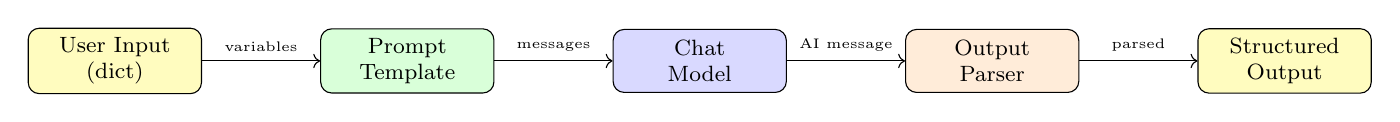
\begin{tikzpicture}[
  node distance=1.5cm,
  box/.style={rectangle, rounded corners, draw, minimum width=2.2cm, minimum height=0.8cm, align=center, font=\footnotesize},
  every edge/.style={draw, -{Stealth[length=5pt]}},
]
  \node[box, fill=yellow!25] (input) {User Input\\(dict)};
  \node[box, fill=green!15, right=of input] (prompt) {Prompt\\Template};
  \node[box, fill=blue!15, right=of prompt] (model) {Chat\\Model};
  \node[box, fill=orange!15, right=of model] (parser) {Output\\Parser};
  \node[box, fill=yellow!25, right=of parser] (output) {Structured\\Output};

  \draw[->] (input) -- (prompt) node[midway, above, font=\tiny] {variables};
  \draw[->] (prompt) -- (model) node[midway, above, font=\tiny] {messages};
  \draw[->] (model) -- (parser) node[midway, above, font=\tiny] {AI message};
  \draw[->] (parser) -- (output) node[midway, above, font=\tiny] {parsed};
\end{tikzpicture}
\end{center}

\vspace{0.2cm}

\begin{conceptbox}[Each Arrow is a Runnable Boundary]
At each step, the output of one Runnable becomes the input of the next. LangSmith tracing captures every boundary for debugging.
\end{conceptbox}
\end{frame}

% ============================================================
\begin{frame}{LangChain vs Alternatives}

\begin{center}
\renewcommand{\arraystretch}{1.2}
\scriptsize
\begin{tabular}{lcccc}
\toprule
\textbf{Feature} & \textbf{LangChain} & \textbf{LlamaIndex} & \textbf{Haystack} & \textbf{Raw SDK} \\
\midrule
Agent framework & \checkmark\checkmark & \checkmark & \checkmark & --- \\
RAG pipeline & \checkmark\checkmark & \checkmark\checkmark\checkmark & \checkmark\checkmark & Manual \\
Provider agnostic & \checkmark\checkmark\checkmark & \checkmark\checkmark & \checkmark\checkmark & --- \\
Graph orchestration & \checkmark\checkmark\checkmark & --- & --- & --- \\
Observability & \checkmark\checkmark\checkmark & \checkmark & \checkmark & Manual \\
Community/ecosystem & \checkmark\checkmark\checkmark & \checkmark\checkmark & \checkmark & N/A \\
Learning curve & Medium & Medium & Medium & Low \\
\bottomrule
\end{tabular}
\end{center}

\vspace{0.15cm}

\begin{tipbox}[Choosing LangChain]
LangChain excels at \textbf{agent orchestration}, \textbf{provider flexibility}, and \textbf{production observability}. LlamaIndex may be better for pure RAG-focused applications.
\end{tipbox}
\end{frame}

% ============================================================
\begin{frame}{What Changed: LangChain v0.x $\rightarrow$ v1.x}

\begin{warningbox}[Breaking Changes in v1.0+]
\begin{itemize}\setlength{\itemsep}{1pt}
  \item \textbf{LCEL is the standard} --- Legacy chains (\texttt{LLMChain}, etc.) moved to \texttt{langchain-classic}
  \item \textbf{Provider packages split out} --- e.g.\ \texttt{from langchain\_openai import ChatOpenAI}
  \item \textbf{langchain-core extracted} --- Interfaces live in \texttt{langchain-core}
  \item \textbf{Agents built on LangGraph} --- \texttt{create\_react\_agent} returns a graph
  \item \textbf{Python 3.10+ required}
\end{itemize}
\end{warningbox}

\vspace{0.1cm}

\begin{tipbox}[Migration Tip]
Start by updating imports to provider-specific packages, then replace legacy chains with LCEL pipelines.
\end{tipbox}
\end{frame}

% ============================================================
\begin{frame}{The Learning Path Ahead}

\begin{center}
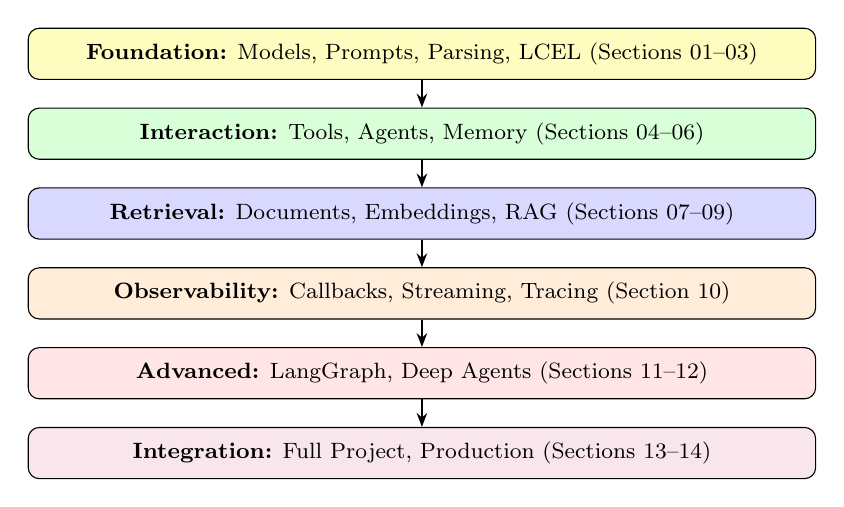
\begin{tikzpicture}[
  node distance=0.35cm,
  phase/.style={rectangle, rounded corners, draw, minimum width=10cm, minimum height=0.65cm, align=center, font=\footnotesize},
]
  \node[phase, fill=yellow!25] (p1) {\textbf{Foundation:} Models, Prompts, Parsing, LCEL (Sections 01--03)};
  \node[phase, fill=green!15, below=of p1] (p2) {\textbf{Interaction:} Tools, Agents, Memory (Sections 04--06)};
  \node[phase, fill=blue!15, below=of p2] (p3) {\textbf{Retrieval:} Documents, Embeddings, RAG (Sections 07--09)};
  \node[phase, fill=orange!15, below=of p3] (p4) {\textbf{Observability:} Callbacks, Streaming, Tracing (Section 10)};
  \node[phase, fill=red!10, below=of p4] (p5) {\textbf{Advanced:} LangGraph, Deep Agents (Sections 11--12)};
  \node[phase, fill=purple!10, below=of p5] (p6) {\textbf{Integration:} Full Project, Production (Sections 13--14)};

  \draw[-{Stealth[length=5pt]}, thick] (p1) -- (p2);
  \draw[-{Stealth[length=5pt]}, thick] (p2) -- (p3);
  \draw[-{Stealth[length=5pt]}, thick] (p3) -- (p4);
  \draw[-{Stealth[length=5pt]}, thick] (p4) -- (p5);
  \draw[-{Stealth[length=5pt]}, thick] (p5) -- (p6);
\end{tikzpicture}
\end{center}
\end{frame}

% ============================================================
\begin{frame}{Summary}

\begin{conceptbox}[Key Takeaways]
\begin{enumerate}\setlength{\itemsep}{1pt}
  \item LangChain is a \textbf{framework for composing LLM-powered applications}, not an LLM itself
  \item The ecosystem spans \textbf{four pillars}: langchain-core, langchain, LangGraph, LangSmith
  \item Everything implements the \textbf{Runnable protocol}: \texttt{invoke()}, \texttt{batch()}, \texttt{stream()}
  \item Components compose with the \textbf{pipe operator} (\texttt{|}) via LCEL
  \item Provider packages are \textbf{separate}: install only what you need
  \item v1.x is a \textbf{major redesign} --- use LCEL, not legacy chains
\end{enumerate}
\end{conceptbox}
\end{frame}

% ============================================================
\begin{frame}[fragile]{Cheat Sheet: Essential Imports}

\begin{codebox}[Imports You'll Use Most Often]
\begin{lstlisting}[basicstyle=\ttfamily\tiny]
# Core
from langchain_core.messages import HumanMessage, AIMessage
from langchain_core.prompts import ChatPromptTemplate
from langchain_core.output_parsers import StrOutputParser
from langchain_core.runnables import RunnablePassthrough
# Models (pick your provider)
from langchain_openai import ChatOpenAI
from langchain_anthropic import ChatAnthropic
# Agents & Tools
from langchain.agents import create_react_agent
from langchain_core.tools import tool
# RAG
from langchain_community.document_loaders import PyPDFLoader
from langchain_text_splitters import RecursiveCharacterTextSplitter
from langchain_openai import OpenAIEmbeddings
from langchain_community.vectorstores import FAISS
\end{lstlisting}
\end{codebox}
\end{frame}

% ============================================================
\begin{frame}{Self-Check Questions}

Test your understanding of this section:

\begin{enumerate}\setlength{\itemsep}{2pt}
  \item What problem does LangChain solve that raw LLM SDKs do not?
  \item Name the four pillars of the LangChain ecosystem and their roles.
  \item What is the Runnable protocol, and why does it matter for composition?
  \item Why are provider packages (e.g., \texttt{langchain-openai}) separate?
  \item What is LCEL and what operator does it use?
  \item How does LangChain v1.x differ from v0.x?
  \item When might you choose \textbf{not} to use LangChain?
\end{enumerate}

\vspace{0.2cm}
\textit{Review any you're unsure about before proceeding to Section 01.}
\end{frame}

\end{document}
